\documentclass[krantz1,ChapterTOCs]{krantz}
\usepackage{fixltx2e,fix-cm}
\usepackage{amssymb}
\usepackage{amsmath}
\usepackage{graphicx}
\usepackage{subfigure}
\usepackage{makeidx}
\usepackage{multicol}
\usepackage{hyperref}
\usepackage{xcolor}

\begin{document}

\section{Exercises-Answer key}

\begin{enumerate}
    \item \begin{align*}
              A &= {1,2,3,4,5,6};
              \;\;B = {1,3,6} \\
              C &= {7}  
              \;\;D = \emptyset
           \end{align*}
    \begin{enumerate}
        \item Please compute $A \cap B$
        \begin{enumerate}
            \item {\color{red} $A \cap B = \{1,3,6  \}$ }
        \end{enumerate}
        \item Please compute $A \cup C$
            \begin{enumerate}
                \item {\color{red} $A \cup C =  \{1,2,3,4,5,6,7\}$}
            \end{enumerate}
        
        \item Please compute $A \cup D$
            \begin{enumerate}
                \item {\color{red} $A \cup D = \{1,2,3,4,5,6\}$  }
            \end{enumerate}
        
        \item Please compute $A \cap D$
            \begin{enumerate}
                \item {\color{red} $A \cap D = \emptyset$  }
            \end{enumerate}
        
        \item Please compute $(A \cap B) \cup (C \cup D)$
            \begin{enumerate}
                \item {\color{red}
                \begin{align*}
                    (A \cap B) \cup (C \cup D) &= \{1,3,6\} \cup \{7\} \\
                    &= \{1,3,6,7\}
                \end{align*}    
                    }
            \end{enumerate}
        
    \end{enumerate}
    \item Let the sample space $\mathcal{G} = \{ 1,2,3,4,5,6,7 \}$
    \begin{enumerate}
       \item Please compute $A^{c}$
           \begin{enumerate}
                \item {\color{red} $A^{c} = \{7\}$  }
            \end{enumerate}
        
       \item Please compute $B^{c}$
           \begin{enumerate}
                \item {\color{red} $B^{c} = \{2,4,5\}$  } 
            \end{enumerate}
        
       \item Please compute $D^{c}$
           \begin{enumerate}
                \item {\color{red} $D^{c} = \{1,2,3,4,5,6,7\}$  }
            \end{enumerate}
        
       \item Please compute $\mathcal{G} \cap A$
           \begin{enumerate}
                \item {\color{red} $ \mathcal{G} \cap A = \{ 1,2,3,4,5,6 \} $  }
            \end{enumerate}
        
       \item Is $A \subset \mathcal{G}$?
           \begin{enumerate}
                \item {\color{red} Yes, every item in A is a item in $\mathcal{G}$  }
            \end{enumerate}
        
       \item Is $\emptyset \subset \mathcal{G}$?
           \begin{enumerate}
                \item {\color{red} Yes, every item (nothing) in the empty set is in $\mathcal{G}$  }
            \end{enumerate}
        
    \end{enumerate}
    
    \item Let the sample space $\samplespace = \{0,1,2,a,b,c\}$ and let $A=\{0,1\}$, $B=\{x | x\text{ is a letter of the English alphabet}\}$
    \begin{enumerate}
        \item Please compute $A \cap B$
            \begin{enumerate}
                \item {\color{red} $ A \cap B =  \emptyset $  }
            \end{enumerate}
        
        \item Please compute $A \cup B$
            \begin{enumerate}
                \item {\color{red} $A \cup B = \{0,1,a,b,c\}$  }
            \end{enumerate}
        
        \item Please compute $A^{c}$
            \begin{enumerate}
                \item {\color{red} $A^{c} = \{2,a,b,c \} $  }
            \end{enumerate}
        
        \item Is $A \cup B = $\mathcal{G}$?
            \begin{enumerate}
                \item {\color{red} No, the item 2 is in $\mathcal{G}$ but this item is not in  $A \cap B$  }
            \end{enumerate}
        
        \item If we assigned probabilities to all outcomes, could $P(A \cup B) = 1$? why or why not?
            \begin{enumerate}
                \item {\color{red} No, only a set that contains all items (the sample space) can equal probability one. Because A union B is not equal to the sample space then it cannot be assigned a probability of one.  }
            \end{enumerate}
        
    \end{enumerate}
    
    \item Let $A = {0,1,2}$ for some sample space $\mathcal{G} = \{0,1,2,3,4,5,6\}$. Further assume $P(A) = 0.2$. 
    \begin{enumerate}
        \item Are the sets $A$ and $A^{c}$ disjoint? Why or why not.
            \begin{enumerate}
                \item {\color{red} Yes, by definition any item in $A$ cannot be an item in $A^{c}$ and so $A \cap A^{c} = \emptyset$}
            \end{enumerate}
        
        \item Simplify $P(A \cup A^{c})$ into an expression that involves $P(A)$ and $P(A^{c})$.
            \begin{enumerate}
                \item {\color{red} 
                \begin{align*}
                    P(A \cup A^{c}) = P(A) + P(A^{c}) & & \text{(Disjoint)}
                \end{align*}
                }
            \end{enumerate}
        
        \item Use Kolmogorov's axioms to show that $P(A) = 1 - P(A^{c})$ 
            \begin{enumerate}
                \item {\color{red}   
                \begin{align*}
                    P(\mathcal{G}) &= P(A \cup A^{c}) & & \text{(Every item is either in or not in A)} \\ 
                    P(\mathcal{G}) &= P(A) + P(A^{c}) & & \text{(Disjoint)} \\
                    1 &= P(A) + P(A^{c}) & & \text{(Probability of sample space)} \\ 
                   P(A)  &= 1 -  P(A^{c})
                \end{align*}
                }
            \end{enumerate}
        
    \end{enumerate}
    
    \item Let $\mathcal{G} = \{x | x\text{ is a positive integer}\}$
    \begin{enumerate}
        \item Are the sets $\emptyset$ and $\mathcal{G}$ disjoint?
            \begin{enumerate}
                \item {\color{red} Yes, the intersection of the empty set and the sample space is empty. }
            \end{enumerate}
        
        \item Simplify $P(\mathcal{G} \cup \emptyset)$ into an expression that involves $P(\mathcal{G})$ and $P(\emptyset)$
            \begin{enumerate}
                \item {\color{red} 
                \begin{align*}
                 P(\mathcal{G} \cup \emptyset) = P(\mathcal{G}) + P(\emptyset) & & \text{(Disjoint)}
                \end{align}
                }
            \end{enumerate}
        
        \item Use Kolmogorov's axioms to show that $P(\emptyset) = 0$
            \begin{enumerate}
                \item {\color{red}
                \begin{align*}
                1 &= P(\mathcal{G} \cup \emptyset) \\ 
                 P(\mathcal{G} \cup \emptyset) &= P(\mathcal{G}) + P(\emptyset) & & \text{(Disjoint)}\\
                1 &= P(\mathcal{G}) + P(\emptyset)\\
                P(\emptyset) &=  P(\mathcal{G}) - 1\\
                P(\emptyset) &=  1 - 1 = 0\\
                \end{align}
                }
            \end{enumerate}
        
    \end{enumerate}
    
    \item If $A=\{1,2,3\}$ and $B = \{2,3,4\}$ and $C = \{1,3\}$
    \begin{enumerate}
        \item Can $P(A) < P(B)$? Why or why not
            \begin{enumerate}
                \item {\color{red} The probability of $A$ could be smaller, but we cannot say for sure because $A$ is not a subset of $B$  }
            \end{enumerate}
        
        \item Can $P(A) < P(C)$? Why or why not
            \begin{enumerate}
                \item {\color{red} No, $C$ is a subset of $A$ and so the probability of $A$ cannot be smaller than the probability of $C$. }
            \end{enumerate}
        
    \end{enumerate}
    \item Use what you know about the intersection, about subsets, and about probability to show that $P(A \cap B) \leq P(A)$. Hint: How are $A \cap B$ and $A$ related?
        \begin{enumerate}
                \item {\color{red}
                \begin{align*}
                 A \cap B \subset A \\ 
                 P(A \cap B) \leq P(A) 
                 \end{align*}
                }
            \end{enumerate}
        
    \item Suppose we wish to study the reemergence of cancer among patients in remition. We collect data on 1,000 patients who are in cancer remition and follow them for 5 years. At five years we are interested in the probability of a second cancer. 
    \begin{enumerate}
        \item Define a sample space $\mathcal{G}$ we can use to assign probabilities to a second cancer and no second cancer.
            \begin{enumerate}
                \item {\color{red} $\mathcal{G} = \{ Yes, No\}$ }
            \end{enumerate}
        
        \item After five years of followup we find that 238 patients experienced a second cancer. Use the frequentist approach to assign probabilities to a second cancer \underline{and} no second cancer.
            \begin{enumerate}
                \item {\color{red}
                \begin{align*}
                    P(Yes) = 238/1000\\
                    P(No) = 762/1000\\
                \end{align*}
                
                }
            \end{enumerate}
        
        \item If you collected data on 2,000 patients do you expect the probability of a second cancer to change? How do you expect the probability to be different for 2,000 patients than with 1,000 patients? 
            \begin{enumerate}
                \item {\color{red} The probability will likely change and i expect that the probability assigned after collecting 2000 patients compared to 1000 patients would more accurately represent the true probability of a second cancer. }
            \end{enumerate}
        
    \end{enumerate}
    
   \item A study (link = \href{here}{https://www.science.org/doi/10.1126/science.abj8222} found that young adults were 32 times more at risk to develop multiple sclerosis (MS) after infection with the Epstein-Barr virus compared to young adults who were not infected by the virus. The experiment enrolled 10 million young adults and observed them for a period of 20 years.
   \begin{enumerate}
       \item Design a sample space if we wish to study outcomes that describe the number of young adults who develop MS. 
           \begin{enumerate}
                \item {\color{red} $\mathcal{G} = \{ 0,1,2,3,\cdots,10 \times 10^{6} \}$  }
            \end{enumerate}
        
       \item Build the event $(E_{1})$ "less than 10\% of young adults develop MS" using set notation.
           \begin{enumerate}
                \item {\color{red} $E_{1} = \{ x | x \leq 10^{6}  \}$ }
            \end{enumerate}
        
       \item Build the event $(E_{2})$ "less than 5\% of young adults develop MS" using set notation.
           \begin{enumerate}
                \item {\color{red} $E_{2} = \{ x | x \leq 5\times 10^{5}  \}$}
            \end{enumerate}
        
       \item Are $E_{1}$ and $E_{2}$ disjoint? Why or why not?
           \begin{enumerate}
                \item {\color{red} No, because $E_{1}$ contains items in $E_{2}$}
            \end{enumerate}
        
       \item Can $P(E_{1}) < P(E_{2})$?
           \begin{enumerate}
                \item {\color{red} No, because $E_{2}$ is a subset of $E_{1}$ }
            \end{enumerate}
    \end{enumerate}
            
          \item Please compute the following
   \begin{enumerate}
       \item $A = \{1,2,3\}$ and $B = \{4,5,6\}$. Please compute $A \times B$ (Answer should be a set of tuples)
       
    \begin{enumerate}
        \item {\color{red} $A \times B = \{ (1,4), (1,5), (1,6), (2,4), (2,5), (2,6), (3,4), (3,5), (3,6) \}$ }
    \end{enumerate}
       
       \item $A = \{1,2,3\}$. Please compute $A \times A$ (Answer should be a set of tuples)
            \begin{enumerate}
                \item {\color{red} $A \times A = \{ (1,1), (1,2), (1,3), (2,1), (2,2), (2,3), (3,1), (3,2), (3,3)  \}$  }
            \end{enumerate}
    
       \item How many elements are in $A \times A$ (looking for a number)
         \begin{enumerate}
           \item {\color{red} From the above problem, there are 9 elements  }
        \end{enumerate}
       
       \item How many elements are in  $A \times A \times A$? (looking for a number)
       
         \begin{enumerate}
           \item {\color{red} There are nine elements in $A \times A$ and there are 3 elements in $A$. Becasue we pair each of the three elements with each of the 9 elements in $A \times A$ there will be 27 elements in $A \times A \times A$  }
         \end{enumerate}
       
       \item How many elements are in  $A \times A \times A \times \cdots \times A$ where we take the Cartesian product $N$ times? (looking for a number)
       
         \begin{enumerate}
           \item {\color{red} We observe the following pattern between cartesian products of $A$ with itself and the number of items: (A,3), ($A \times A$, $3 \cdot 3= 3^{2}$), ($A \times A \times A$, $3 \cdot 3 \cdot 3 = 3^3}$)  , and so we expect there to be $3^{N}$ elements in the cartesian product of $A$ with itself $N$ times.}
         \end{enumerate}
       
   \end{enumerate}
   \item Define a sample space $\samplespace = \{ a,b,c,d,1,2,3,4,5 \}$ and let $E_{1} = \{1,3,5\}$, $E_{2} = \{a,b,c\}$, $E_{3} = \{ a,d,5 \}$. We further assign the following probabilities 
   \begin{table}[ht!]
       \centering
       \begin{tabular}{ c c}
       Outcome &  $P(\{\text{Outcome}\})$\\
       \hline
            a & 0.10  \\
            b & 0.05 \\
            c & 0.15 \\
            d & 0.02 \\
            1 & 0.14 \\
            2 & 0.25 \\
            3 & 0.08 \\
            4 & 0.04 \\
            5 & 0.17
       \end{tabular}
   \end{table}
   \begin{enumerate}
       \item Compute $P(E_{1})$ (looking for a number)
       \begin{enumerate}
           \item {\color{red} $P(E_{1}) = P(\{1\}) + P(\{3\}) + P(\{5\}) = 0.14 + 0.08 + 0.17 = 0.39$  }
       \end{enumerate}
       \item Compute $P(E_{2})$ (looking for a number)
       \begin{enumerate}
           \item {\color{red}  P(E_{2}) = P(\{a\}) + P(\{b\}) + P(\{c\}) = 0.10 + 0.05 + 0.15 = 0.30 }
       \end{enumerate}
       \item Compute $P(E_{3})$ (looking for a number)
       \begin{enumerate}
           \item {\color{red}  P(E_{3}) = P(\{a\}) + P(\{d\}) + P(\{5\}) = 0.10 + 0.02 + 0.17 = 0.29 }
       \end{enumerate}
       \item Compute $P(E_{1} \cap E_{2})$ (looking for a number)
       \begin{enumerate}
           \item {\color{red} P(E_{1} \cap E_{2}) = P(\emptyset) = 0  }
       \end{enumerate}
       \item Compute $P(E_{1} \cap E_{3})$ (looking for a number)
       \begin{enumerate}
           \item {\color{red}  P(E_{1} \cap E_{3}) = P(\{5\}) = 0.17}
       \end{enumerate}
       \item Compute $P(E_{2} \cap E_{3})$ (looking for a number)
       \begin{enumerate}
           \item {\color{red}  P(E_{2} \cap E_{3}) = P(\{a\}) = 0.10}
       \end{enumerate}
       \item Compute $P(E_{1} | E_{2})$ (looking for a number)
       \begin{enumerate}
           \item {\color{red}  $\frac{P(E_{1} \cap E_{2})}{P(E_{2})}$ = 0 / 0.30 = 0 }
       \end{enumerate}
       \item Compute $P(E_{1} | E_{3})$ (looking for a number)
       \begin{enumerate}
           \item {\color{red} $P(E_{1} \cap E_{3}) / P(E_{3}) = 0.17 / 0.29 = 0.586$   }
       \end{enumerate}
       \item Compute $P(E_{2} | E_{3})$ (looking for a number)
       \begin{enumerate}
           \item {\color{red}  $P(E_{2} \cap E_{3}) / P(E_{3}) = 0.10 / 0.29 = 0.344$  }
       \end{enumerate}
       \item Compute $P(E_{3} | E_{2})$ (looking for a number)
       \begin{enumerate}
           \item {\color{red} $P(E_{3} \cap E_{2}) / P(E_{2}) = 0.10 / 0.30 = 0.333$  }
       \end{enumerate}
   \end{enumerate}
   \item Define a sample space $\samplespace = \{ (a,1),(b,1),(c,1),(a,2),(b,2),(c,2) \}$ and let $E_{1} = \{(a,1),(a,2),(c,2)\}$, $E_{2} = \{(c,2),(a,1) \}$, $E_{3} = \{(b,2) \}$. We further assign the following probabilities 
   \begin{table}[ht!]
       \centering
       \begin{tabular}{ c c}
       Outcome &  $P(\{\text{Outcome}\})$\\
       \hline
            (a,1) & 0.05  \\
            (b,1) & 0.22 \\
            (c,1) & 0.15 \\
            (a,2) & 0.02 \\
            (b,2) & 0.13 \\
            (c,2) & 0.43 \\
       \end{tabular}
   \end{table}
   \begin{enumerate}
       \item Compute $P(E_{1})$ (looking for a number)
       \begin{enumerate}
           \item {\color{red} $P(E_{1}) = P(\{(a,1)\})+P(\{(a,2)\}) + P(\{(c,2)\}) = 0.05+0.02+0.43 = 0.50$    }
       \end{enumerate}
       \item Compute $P(E_{2})$ (looking for a number)
       \begin{enumerate}
           \item {\color{red}  $P(E_{2}) = P(\{(c,2)\})+P(\{(a,1)\}) = 0.43 + 0.05 = 0.48 $   }
       \end{enumerate}
       \item Compute $P(E_{3})$ (looking for a number)
       \begin{enumerate}
           \item {\color{red}  $P(E_{3}) = P(\{(b,2)\}) = 0.13 $    }
       \end{enumerate}
       \item Compute $P(E_{1} \cap E_{2})$ (looking for a number)
       \begin{enumerate}
           \item {\color{red} $P(\{ (a,1), (c,2) \} ) = 0.48$    }
       \end{enumerate}
       \item Compute $P(E_{1} \cap E_{3})$ (looking for a number)
       \begin{enumerate}
           \item {\color{red} $P(\{ \}) = 0$     }
       \end{enumerate}
       \item Compute $P(E_{2} \cap E_{3})$ (looking for a number)
       \begin{enumerate}
           \item {\color{red}  $P(\emptyset) = 0$   }
       \end{enumerate}
       \item Compute $P(E_{1} | E_{2})$ (looking for a number)
       \begin{enumerate}
           \item {\color{red} $P(E_{1} \cap E_{2} ) / P(E_{2}) = 0.48/0.48 = 1$     }
       \end{enumerate}
       \item Compute $P(E_{1} | E_{3})$ (looking for a number)
       \begin{enumerate}
           \item {\color{red}  $P(E_{1} \cap E_{3} ) / P(E_{3}) = 0/0.13 = 0$   }
       \end{enumerate}
       \item Compute $P(E_{2} | E_{3})$ (looking for a number)
       \begin{enumerate}
           \item {\color{red}  $P(E_{2} \cap E_{3} ) / P(E_{3}) = 0/0.13 = 0$   }
       \end{enumerate}
       \item Compute $P(E_{3} | E_{2})$ (looking for a number)
       \begin{enumerate}
           \item {\color{red}  $P(E_{2} \cap E_{3} ) / P(E_{2}) = 0/0.48 = 0$    }
       \end{enumerate}
   \end{enumerate}
   
   \item Given two events $A$ and $B$, show that $P(A|B) \geq P(A \cap B)$ (looking for a short explanation and mathematical argument)
   \begin{enumerate}
           \item {\color{red} 
           \begin{align}
               P(A|B) &= \frac{P(A \cap B)}{P(B)}\\
               & 0 \leq P(B) \leq 1 \text{ so }\\
               &\frac{P(A \cap B)}{P(B)} \geq P(A \cap B)
           \end{align}     }
       \end{enumerate}
   
   \item Suppose we wish to study adverse outcomes among patients who have unprotected left main disease~(\url{https://www.nejm.org/doi/full/10.1056/nejmoa1909406}). In this experiment~(called a clinical trial) we randomize patients to receive percutaneous intervention~(PCI) or a coronary artery bypass graft~(CABG). We wish to study the number of patients who received a PCI \underline{and} experienced a myocardial infarction~(MI) between the time they had their procedure and 5 years, however we only know three pieces of information: (i) the probability a patient was randomized to PCI was 0.5, (ii) the probability a patient was randomized to CABG was 0.5, and (iii) we know that the probability of a MI was 0.2 among patients who received a PCI.
   \begin{enumerate}
       \item Define a sample space that will allow us to compute the probability a patient was randomized to PCI and experienced an MI (looking for a description of the sample space and a set)
       \begin{enumerate}
           \item {\color{red}  $\mathcal{G} = \{(PCI,MI),(No PCI,MI),(PCI, No MI),(No PCI, No MI)\}$   }
       \end{enumerate}
       \item Please compute the probability a patient experiences an MI and was randomized to PCI. (looking for a number)
       \begin{enumerate}
           \item {\color{red}  
           \begin{align}
               &MI = \{ (PCI,MI),(No PCI, MI) \} \\ 
               &PCI = \{ (PCI,MI),(PCI, No MI) \} \\
               &P(PCI \cap MI) = P(MI | PCI) P(PCI) &  \text{multiplication rule}    \\
              & 0.2 \times 0.5 = 0.1 
           \end{align}   }
       \end{enumerate}
       \item Please compute the probability a patient does not experience an MI and was randomized to PCI. (looking for a number)
       \begin{enumerate}
           \item {\color{red}  P(PCI \cap No MI) = P(No MI | PCI) P(PCI)   }  = $0.8 \times 0.5 &= 0.4$ 
       \end{enumerate}
   \end{enumerate}
   
   \item If two events $A$ and $B$ are disjoint, are they also independent? (looking for a description and mathematical argument to backup your description.)
   \begin{enumerate}
        \item {\color{red} No. Suppose we build two sets $A$ and $B$ that are disjoint and non empty (they contain outcomes). Then $P(A|B) = P(A \cap B) / P(B) = 0/P(B) = 0 $. However $P(A) > 0$ and so $P(A|B) \neq P(A)$      }
    \end{enumerate}
   
   \item Researchers studied epidemiological characteristics of a variant of SARS-CoV-2 called B.1.526~(\url{https://www.science.org/doi/10.1126/sciadv.abm0300}). Suppose we too wanted to study the impact of B.1.526 on a population of patients who have been admitted to the hospital for COVID-19 by collecting each patient's age, whether they have were vaccinated against COVID-19, and whether their infection was due to the B.1.526 variant.
   
   \begin{enumerate}
       \item If we define our experiment as generating the above three pieces of information from a single patient, define a sample space~($\samplespace$) for these potential outcomes. (looking for a short description and the sample space)
       \begin{enumerate}
           \item {\color{red}     }
       \end{enumerate}
       \item Define a sample space if we repeated our above experiment 2 times. In other words, what would be our sample space if we collected information from 2 patients? 
       \begin{enumerate}
           \item {\color{red}     }
       \end{enumerate}
   \end{enumerate}
    
   \item Can a data set ever have more elements than a sample space? Explain. (looking for a paragraph with some examples)
   \begin{enumerate}
           \item {\color{red}     }
       \end{enumerate}
   
   \item Suppose we collect the following data about the co-occurence of patients admitted to the hospital for influenza-like illness~(ILI) and whether the patient does or does not work in a clinical setting. 
   After data collection we estimate the following probabilities: The probability that a patient works in a clinical setting is 0.12. The probability that a patient who works in a clinical setting is admitted to the hospital for ILI is 0.2, and the probability a patient who does not work in a clinical setting was admitted to the hospital for ILI is 0.3. 
   \begin{enumerate}
       \item Define a sample space to study outcomes related to the co-occurance of ILI/No ILI and patients who do/do not work in a clinical setting. (Looking for a set and a very brief description of an outcome or two.) 
       \item Compute the probability a patient is admitted to the hospitals for ILI and they work in a clinical setting. (Looking for an equation and number)
       \item Compute the probability a patient is not admitted to the hospital for ILI and they work in a clinical setting. (Looking for an equation and number)
       \item Compute the probability a patient is admitted to the hospital for ILI and they do not work in a clinical setting. (Looking for an equation and number)
       \item Compute the probability a patient is not admitted to the hospital for ILI and they do not work in a clinical setting. (Looking for an equation and number)
   \end{enumerate}
   
   \item Show that for two events $A$ and $B$ the $P(A|B)P(B)  \leq P(B)$. Why is this the case intuitively? (Looking for two brief descriptions)
   \clearpage
   \item \begin{figure}[ht!]
       \centering
       \fbox{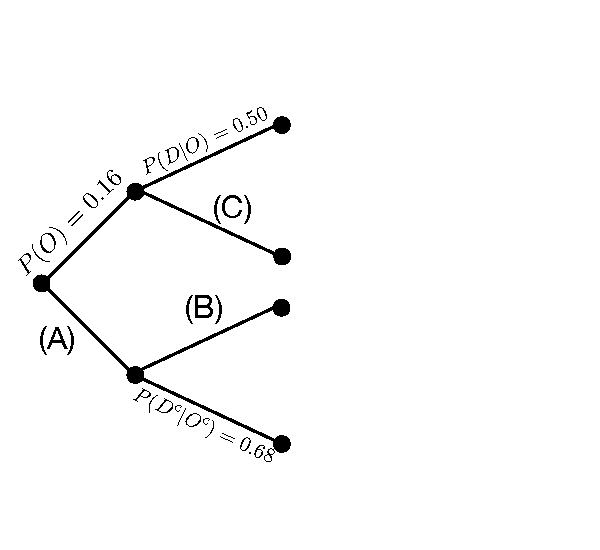
\includegraphics{chapters/chapter1/tree_diagram__HW.pdf}}
   \end{figure} Please use the above tree diagram to answer the following questions. 
   \begin{enumerate}
       \item Fill in the $P(O^{c})$ which corresponds to (A) in the figure
       \item Fill in the $P(D | O^{c})$ which corresponds to (B) in the figure
       \item Fill in the $P(D^{c} | O)$ which corresponds to (C) in the figure
       \item Please compute $P(D)$
       \item Please compute $P(D^{c})$
   \end{enumerate}
   
   \item Influenza is a contagious virus that enters the respiratory system from a human's nose, throat, or lungs. Common symptoms are cough, chills, and a fever.
   Suppose we collect data from a local hospital about those who were infected and not infected by the influenza virus and the above three symptoms. Let $\samplespace = \{ (x,y)  | x \text{ is } \text{"Flu"} \text{ or } \text{"not Flu"} \text{ and } y \in \{ \text{cough },\text{chills },\text{ fever} \}   \}$. 
   Suppose further that we define events $F$ = \{ (x,y)  | x \text{ is } \text{"Flu"} \}, $C$ = \{ (x,y)  | y \text{ is } \text{"Cough"} \}, $H$ = \{ (x,y)  | y \text{ is } \text{"Chills"} \} , $E$ = \{ (x,y)  | y \text{ is } \text{"Fever"} \}, and that $P( C|F ) = 0.5$ and $P( C|F^{c} ) = 0.15$, $P( H|F ) = 0.25$ and $P( H|F^{c} ) = 0.01$, $P( E|F ) = 0.98$ and $P( E|F^{c} ) = 0.35$, $P(F) = 0.02$  
    \begin{enumerate}
       \item A patient presents with the chills. What is the probability they have influenza? 
       \item What symptom from the above, if present, would indicate with a high probability a patient has influenza?
    \end{enumerate}
 
            
        
   \end{enumerate}
    
\end{document}
